\chapter{Game Theory}\label{ch:gametheory}

\section{Games}\label{sec:games}

Game theory studies decision problems in which the outcome of an agent's choice
depends on other agents' choices. Such problems are called \textbf{games}, and
the agents \textbf{players}. The Prisoner's Dilemma (example \ref{ex:pd}) is a
game in this sense, because the outcome of your choice (confessing or remaining
silent) depends on what your partner decides to do.

Whenever an agent faces a choice in a game, the MEU Principle tells us that they
ought to choose whichever option maximizes expected utility. We don't need a new
decision theory for games. Nonetheless, there are reasons for studying the
special case where the states in a decision problem are other people's (real or
potential) actions.

One reason is that we may be able to shed light on important social and
political issues. The way we live and behave, as a society, is in many ways not
ideal. We are depleting the Earth's resources. We are destabilising the climate.
We are woefully underprepared for pandemics and other catastrophes. We buy goods
from online retailers where most of the products are a scam. Corruption is
rampant. The political system is broken. Dating is broken. And so on, and on.
Why? Why don't we fix these problems? Is it because the current system benefits
powerful actors who have us under their control? Game theory suggests an
alternative possibility.

Remember the Prisoner's Dilemma. If you and your partner are rational and don't
care about each other, you both confess and spend a long time in prison.
Collectively, you could have achieved a much better outcome by remaining silent.
Things are unnecessarily bad -- you spend a long time in prison -- not because a
powerful third party stands to gain from your misery. The bad outcome is simply
a result of your misaligned incentives.

This kind of situation is sadly common. Professional athletes, for example, have
a strong incentive to use steroids, as long as the chance of being caught is
low. Whether or not their competitors do the same, using steroids provides an
advantage. The outcome is that everyone uses steroids, even though everyone
would prefer that no-one uses steroids. Structurally, the athletes' decision
problem is the same as the Prisoner's Dilemma. Any decision problem with this
structure is nowadays called a Prisoner's Dilemma, even if no prisoners are
evolved.

Another famous example is the ``tragedy of the commons''. Fishermen have an
incentive to catch as many fish as they can, even though everyone would be
better off if everyone restrained themselves to sustainable quotas.

Thomas Hobbes (in effect) argued that the pervasiveness of Prisoner's Dilemmas
justifies the subordination of people under a state. It is in everyone's
interest to impose a system of control and punishment that ensures the best
outcome in what would otherwise be a Prisoner's Dilemma.

\begin{exercise}{1}
  How do criminal organisations like the Mafia ensure that its members remain
  silent when they are interrogated by the police? Draw the decision matrix for
  the scenario of the (original) Prisoner's Dilemma, but assuming that both
  players are members of the Mafia.
\end{exercise}

Another reason to study games is that a new set of conceptual tools and
techniques become available if the states in a decision problem are other
people's actions. In particular, we can often figure out which state obtains
based on the other players' desires. In the original Prisoner's Dilemma, we
know that if your partner is rational any only cares about their own prison term
then they will confess.

Here is how game theorists would typically draw the matrix for the Prisoner's
Dilemma, assuming you and your partner don't care about each other:
%
\begin{dmatrix}{r|c|c} & Confess & Silent\\\hline Confess & -5, -5 & 0, -8
\\\hline Silent & -8, 0 & -1, -1 \\\hline
\end{dmatrix}
%
As before, the rows are the acts available to you. The columns are the acts
available to your partner. We generally don't assign credences to the columns.
The numbers in the cells represent the utility of the relevant outcome for you
and your partner. We don't describe the outcome itself any more, for lack of
space. The first number in each cell is the utility for the row player (whom
we'll call `Row' and assume to be female); the second is the utility for the
column player (`Column', male).

In game theory jargon, a \textbf{solution} to a game is a prediction of what
each player is going to do, assuming that they are rational. The solution to the
Prisoner's Dilemma is that each player confesses. Confessing dominates remaining
silent. You should confess no matter what you think your partner will do.

% \begin{exercise}{1}
%   Draw the game matrix for the Prisoner Dilemma, assuming you
%   only care about your own prison term, but your partner cares equally
%   about both of you.
% \end{exercise}

Consider the following matrix, for a different kind of game. 

\begin{dmatrix}{r|c|c}
   &  $C_1$ &  $C_2$ \\\hline
   $R_1$ & 2, 2 & 1, 3 \\\hline
   $R_2$ & 1, 1 & 2, 2 \\\hline
\end{dmatrix}
\noindent%
Row no longer has a dominant option. What she should do depends on what she
thinks Column will do. If Column chooses $C_1$, then Row should play $R_1$; if
Column chooses $C_2$, then Row should play $R_2$. Can we nonetheless say what
Row will do, without specifying her beliefs?

Look at the game from Column's perspective. No matter what Row does, Column is
better off choosing $C_2$. $C_2$ dominates $C_1$. So if Row knows the utility
that Column assigns to the outcomes, then she can figure out that Column will
choose $C_2$. And so Row should choose $R_2$. The solution is $R_2, C_2$: Row
chooses $R_{2}$ and Column $C_{2}$.

Here is another, more complex example.
\begin{dmatrix}{r|c|c|c}
     &  $C_1$ &  $C_2$ &  $C_3$ \\\hline
     $R_1$ & 0, 1 & 2, 2 & 3, 1 \\\hline
     $R_2$ & 2, 2 & 1, 3 & 2, 2 \\\hline
     $R_3$ & 1, 1 & 0, 2 & 0, 3 \\\hline
\end{dmatrix}
\noindent%
From Row's perspective, $R_1$ is the best choice if Column plays $C_2$ or $C_3$,
and $R_2$ is the best choice if Column goes for $C_1$. For Column, $C_2$ is the
best choice in case of $R_1$ or $R_2$, and $C_3$ is best in case of $R_3$. But
Column can hardly expect Row to choose $R_3$, since $R_3$ is dominated by $R_2$.
Column can figure out that Row will play either $R_1$ or $R_2$, which means
that Column will play $C_2$. And since Row can figure out that Column will play
$C_2$, Row will play $R_1$. The solution is $R_1, C_2$.

To reach this conclusion, we need to assume more than that both players know
each other's utilities. To figure out that Column will play $C_2$, Row needs to
know that Column knows her (Row's) utilities, and she needs to know that Column
knows that she (Row) won't choose a dominated option.

A common idealisation in game theory is that the players have \textbf{complete
  information} about the game, meaning that
\begin{enumerate*}
  \itemsep0em
  \item[(1)] all players know the structure of the game, as displayed in the
  matrix;
  \item[(2)] all players know that all players are rational;
  \item[(3)] all players know that (1)--(3) are satisfied.
\end{enumerate*}
By applying to itself, the clause (3) ensures that (1) and (2) hold with
arbitrarily many iterations of `all players know that' stacked in front. If
something is in this way known by everyone, and known by everyone to be known by
everyone, and so on, then it is said to be \textbf{common knowledge}. (1)--(3)
say that the structure of the game and the rationality of all participants are
common knowledge.

\begin{exercise}{2}\label{e:elim-dom-strat}
  Under the assumptions (1)--(3), what will Row and Column do in the following games?
  \medskip

  \begin{minipage}[t][\parskip][t]{0.3\textwidth}
    a.\\
    \begin{inlinedmatrix}{r|c|c}
      &  $C_1$ &  $C_2$ \\\hline
      $R_1$ & 1, 0 & 1, 2  \\\hline
      $R_2$ & 0, 3 & 0, 1 \\\hline
    \end{inlinedmatrix}
  \end{minipage}
  \begin{minipage}[t][\parskip][t]{0.37\textwidth}
    b.\\
    \begin{inlinedmatrix}{r|c|c|c}
      & $C_1$ & $C_2$ & $C_3$ \\\hline
      $R_1$ & 1, 0 & 1, 2 & 0, 1 \\\hline
      $R_2$ & 0, 3 & 0, 1 & 2, 0 \\\hline
      \end{inlinedmatrix}
    \cmnt{%
    $C_3$ is dominated by $C_2$; having removed $C_3$, $R_2$ is dominated by $R_1$.
    } %
  \end{minipage}
  \begin{minipage}[t][\parskip][t]{0.3\textwidth}
    c.\\
    \begin{inlinedmatrix}{r|c|c|c}
          &  $C_1$ &  $C_2$ &  $C_3$ \\\hline
          $R_1$ & 0, 1 & 2, 0 & 2, 4 \\\hline
          $R_2$ & 4, 3 & 1, 4 & 2, 5 \\\hline
          $R_3$ & 2, 4 & 3, 6 & 3, 1 \\\hline
      \end{inlinedmatrix}
      \cmnt{%
        $R_1$ is dominated by $R_3$; then $C_1$ by $C_2$; then $R_2$ by $R_3$. So R2,C3.
      } %
  \end{minipage}
  \vspace{2.8cm}

\end{exercise}

\section{Nash equilibria}

Have a look at this game.

\begin{dmatrix}{r|c|c|c}
    &  $C_1$ &  $C_2$ &  $C_3$ \\\hline
    $R_1$ & 4, 2 & 2, 3 & 2, 3 \\\hline
    $R_2$ & 2, 1 & 3, 2 & 4, 1 \\\hline
    $R_3$ & 3, 3 & 1, 1 & 4, 2 \\\hline
\end{dmatrix}
\noindent%
No option for either player is dominated by any other. Can we nonetheless figure
out what Row and Column will choose?

Let's start with some trial and error. Take $R_1, C_1$. Could this be how the
game is always played, under the idealizing assumptions (1)--(3)? No. Otherwise
Column would know that Row is going to play $R_1$. And then Column is better off
playing $C_2$ or $C_{3}$. What about $R_1, C_2$? If this is how the game has to
played, then Row would know that Column plays $C_2$, and then she would be
better off playing $R_2$. This kind of reasoning disqualifies all combinations
except $R_2, C_2$ -- the middle cell. If Row knows that Column is going to play
$C_2$, she can do no better than play $R_2$. Likewise for Column: if Column
knows that Row is going to play $R_2$, he can do no better than play $C_2$.

A combination of options that is ``stable'' in this way is called a \textbf{Nash
  equilibrium} (after the economist John Nash). In general, a Nash equilibrium
is a combination of acts, one for each player, such that no player could get
greater utility by deviating from their part of the equilibrium, given that the
other players stick to their part.

There is a simple algorithm for finding Nash equilibria in two-player games.
Start from the perspective of the row player. For each act of the column player,
underline the best outcome(s) Row can achieve if Column chooses this act. In the
example above, you would underline the 4 in the first column, the 3 in the
middle cell, and both 4s in the third column. Then do the same for the column
player: for each act of Row, underline the best possible outcome(s) for Column.
The result looks like this.
\begin{dmatrix}{r|c|c|c}
    &  $C_1$ &  $C_2$ &  $C_3$ \\\hline
    $R_1$ & \underline{4}, 2 & 2, \underline{3} & 2, \underline{3} \\\hline
    $R_2$ & 2, 1 & \underline{3}, \underline{2} & \underline{4}, 1 \\\hline
    $R_3$ & 3, \underline{3} & 1, 1 & \underline{4}, 2 \\\hline
\end{dmatrix}
Any cell in which both numbers are underlined is a Nash equilibrium.

A common assumption in game theory is that if a game has a unique Nash
equilibrium, and assumptions (1)--(3) are satisfied, then the Nash equilibrium
is the game's solution: each player will play their part of the equilibrium.

But this isn't obvious. Our trial-and-error reasoning from above shows that
\emph{if a game has a unique solution}, and assumptions (1)--(3) are satisfied,
\emph{then the solution is a Nash equilibrium}. The reason is that if a
game has a unique solution, then (1)--(3) entail that each player knows that the
other will play their part of the solution. Each player plays their part of the
solution with the full knowledge that the other player is playing their
part. So the solution must be a Nash equilibrium.

It doesn't follow, however, that if a game has a unique Nash equilibrium, then
this is the game's solution. Consider the following game.
\begin{dmatrix}{r|c|c|c}
    &  $C_1$ &  $C_2$ &  $C_3$ \\\hline
    $R_1$ & \underline{2}, -2 & -1, \underline{1} & \underline{1}, -1 \\\hline
    $R_2$ & 0, 0 & \underline{0}, 0 & -2, \underline{2} \\\hline
    $R_3$ & 0, \underline{0} & \underline{0}, \underline{0} & \underline{1}, -1 \\\hline
\end{dmatrix}
There is a unique Nash equilibrium: $R_3, C_2$. If this is the guaranteed
outcome under assumptions (1)--(3), then Row can be sure that Column will play
$C_2$. But if Column plays $C_2$, then $R_2$ and $R_3$ are equally good for Row.
So how can we be sure Row won't play $R_{2}$?

You might argue that if Row played $R_2$ and Column could predict her choice,
then Column would play $C_3$, leading to a worse result for Row. But we're not
assuming that Column can predict Row's choice. All we're assuming is (1)--(3).

A better argument in support of $R_{3}, C_{2}$ as the unique solution goes as
follows. Suppose for reductio that Row could play either $R_{3}$ or $R_2$, and
conditions (1)--(3) are satisfied. Then Column can't be sure that Row will play
$R_{2}$. If Column gives equal credence to $R_2$ and $R_3$, then his best choice
is $C_{3}$. And then Row should choose $R_3$, contradicting our assumption that
Row can play $R_2$.

This argument is still a little shaky. Why would Column have to give equal
credence to $R_{2}$ and $R_{3}$? Why couldn't Column be confident that Row will
play $R_{3}$ and yet Row actually plays $R_{2}$?

We need more than (1)--(3) to ensure that a unique Nash equilibrium will always
be played. We seem to need the further assumption that each player can replicate
the other's process of deliberation -- or at least the end point of the process.

One reason to think that this assumption might be satisfied is that the players
seem to have the same evidence about the game. If the norms of rationality
determine how, say, Column should figure out what he should do, based on his
evidence and his goals, then Row -- knowing Column's evidence, his utilities,
and his rationality -- can replicate Column's process of deliberation: she can
figure out how Column will figure out what he should do.

Another, simpler, reason why each player may know about the other's deliberation
is that they have played the same game before. In repeated plays, each player
has direct evidence about how the other tends to play, from what they did on the
previous iterations. If, in the above example, Row always plays $R_{2}$, then
Column will start playing $C_{2}$. Seeing that Column plays $C_{2}$, Row should
switch to $R_{1}$ or $R_{3}$. Eventually, we would expect them to end up in the
Nash equilibrium $R_{3},C_{2}$.


\begin{exercise}{1}\label{e:ne}
  Identify the Nash equilibria in the following games.
  \medskip
  
  \begin{minipage}[t][\parskip][t]{0.29\textwidth}
    a.\\
       \begin{inlinedmatrix}{r|c|c}
         &  $C_1$ &  $C_2$  \\\hline
         $R_1$ & 3, 4 & 4, 3  \\\hline
         $R_2$ & 1, 3 & 5, 2  \\\hline
         $R_3$ & 2, 0 & 1, 5  \\\hline
      \end{inlinedmatrix} 
  \end{minipage}
  \begin{minipage}[t][\parskip][t]{0.37\textwidth}
    b.\\
    \begin{inlinedmatrix}{r|c|c|c}
         &  $C_1$ &  $C_2$ &  $C_3$ \\\hline
         $R_1$ & 1, 0 & 1, 2 & 0, 1 \\\hline
         $R_2$ & 0, 3 & 0, 1 & 2, 0 \\\hline
    \end{inlinedmatrix}
      \cmnt{%
        $C_3$ is dominated by $C_2$; having removed $C_3$, $R_2$ is dominated by $R_1$.
      } %
  \end{minipage}
  \begin{minipage}[t][\parskip][t]{0.3\textwidth}
    c.\\
      \begin{inlinedmatrix}{r|c|c|c}
         &  $C_1$ &  $C_2$ &  $C_3$ \\\hline
         $R_1$ & 0, 1 & 2, 0 & 2, 4 \\\hline
         $R_2$ & 4, 3 & 1, 4 & 2, 5 \\\hline
         $R_3$ & 2, 4 & 3, 6 & 3, 1 \\\hline
      \end{inlinedmatrix}
      \cmnt{%
        $R_1$ is dominated by $R_3$; then $C_1$ by $C_2$; then $R_2$ by $R_3$. So R2, C3.
      } %
  \end{minipage}

  \vspace{2.9cm}
    
\end{exercise}

\begin{exercise}{2}
  Whenever the method from section \ref{sec:games}, which is called
  \textbf{elimination of dominated strategies}, identifies a
  combination of acts as a game's solution, then this combination of
  acts is a Nash equilibrium. Can you explain why?
\end{exercise}

\section{Zero-sum games}

In some games, the players' preferences are exactly opposed: if Row prefers one
outcome to another by a certain amount, then Column prefers the second outcome
to the first by the same amount. The utilities in every cell sum to the same
number. Since utility scales don't have a fixed zero, we can re-scale the
utilities so that the sum is zero. For this reason, games in which the players'
preferences are opposed are called \textbf{zero-sum games}. Here is an example.


\begin{dmatrix}{r|c|c|c}
    &  $C_1$ &  $C_2$ &  $C_3$ \\\hline
    $R_1$ & 1, \underline{-1} & \underline{3}, -3 & \underline{1}, \underline{-1} \\\hline
    $R_2$ & \underline{2}, -2 & -2, \underline{2} & -1, 1 \\\hline
\end{dmatrix}

There is a unique Nash equilibrium: $R_1, C_3$. Curiously, this equilibrium will
be reached if each player follows the \emph{maximin} rule that we've met in
section \ref{sec:solving}. Maximin says to choose an option with the best
worst-case result. In our example, the worst-case result of choosing $R_1$ (for
Row) has utility 1; the worst-case result of $R_2$ is -2. Maximin therefore says
that Row should choose $R_1$. For Column, it similarly recommends $C_3$.

This is not a coincidence. Every Nash equilibrium in every zero-sum game is
supported by the maximin rule. For suppose that $R_{i},C_{j}$ is a Nash
equilibrium in a (two-player) zero-sum game, but $R_{i}$ isn't supported by the
Maximin rule. Then there is an alternative $R_{k}$ whose worst-case outcome is
better for Row than the outcome of $R_{i},C_{j}$. Then every possible outcome of
$R_{k}$ is better for Row than $R_{i},C_{j}$. But if $R_{i},C_{j}$ is a Nash
equilibrium, then $R_{k},C_{j}$ can't be better for Row than $R_{i},C_{j}$.

One might argue that even though maximin is not a generally defensible decision
rule, it makes sense in a zero-sum game with complete information. The idea
would be that whatever option $R_{i}$ Row chooses, she can be confident that
Column will choose an option $C_{j}$ that leads to the best outcome when
combined with $R_{i}$. And the best outcome for Column is the worst outcome for
Row. Like the argument for Nash equilibria in the previous section, however,
this argument assumes that the players can replicate each other's reasoning.

% It doesn't follow that maximin is a sensible rule in for zero-sum games, or
% even that every combination of maximin strategies is a Nash equilibrium.
% Consider an asymmetric version of matching pennies.

Many games have more than one Nash equilibrium. The hypothesis that players
usually end up in a Nash equilibrium then doesn't fully tell us what the players
will do. Here is an example.
\begin{dmatrix}{r|c|c|c}
    &  $C_1$ &  $C_2$ &  $C_3$ \\\hline
    $R_1$ & 2, -2 & \underline{1}, \underline{-1} & \underline{1}, \underline{-1} \\\hline
    $R_2$ & \underline{3}, -3 & \underline{1}, \underline{-1} & \underline{1}, \underline{-1} \\\hline
    $R_3$ & 0, 0 & -1, 1 & -2, \underline{2} \\\hline
\end{dmatrix}
\noindent%
There are fur Nash equilibria. What will the players do? Should Row play $R_1$
or $R_2$? Should Column play $C_2$ or $C_3$? Well, it doesn't matter. The
players can arbitrarily choose among these options. Whatever they choose, they
are guaranteed to end up at an equilibrium, and all the equilibria have the same
utility.

\begin{exercise}{3}
  Prove that this holds for all two-player zero-sum games: if $R_i, C_j$ and
  $R_n, C_m$ are Nash equilibria, then so are $R_i, C_m$ and $R_n, C_j$;
  moreover, all Nash equilibria have the same utility.
\end{exercise}

Some games have no Nash equilibrium at all. Here is a matrix for
Rock--Paper--Scissors.
%
\begin{dmatrix}{r|c|c|c}
    &  Rock &  Paper &  Scissors \\\hline
    Rock & 0, 0 & -1, \underline{1} & \underline{1}, -1 \\\hline
    Paper & \underline{1}, -1 & 0, 0 & -1, \underline{1} \\\hline
    Scissors & -1, \underline{1} & \underline{1}, -1 & 0, 0 \\\hline
\end{dmatrix}
%
There is no equilibrium. What should you do in this kind of game?

A standard answer in game theory is that you should randomize. You should, say,
toss a fair die and choose Rock on 1 or 2, Paper on 3 or 4, and Scissors on 5 or
6. Such a randomized choice is called a \textbf{mixed strategy}. We will write
`[$\nicefrac{1}{3}$ Rock, $\nicefrac{1}{3}$ Paper, $\nicefrac{1}{3}$ Scissors]'
for the mixed strategy of playing Rock, Paper, or Scissors each with (objective)
probability $\nicefrac{1}{3}$.

Suppose two players both play [$\nicefrac{1}{3}$ Rock, $\nicefrac{1}{3}$ Paper,
$\nicefrac{1}{3}$ Scissors]. Then neither could do better by playing anything
else (including other mixed strategies). The combination of the two mixed
strategies is a Nash Equilibrium. It is the only Nash Equilibrium in
Rock--Paper--Scissors.

It can be shown that every finite game has at least one Nash Equilibrium if
mixed strategies are included. (This was shown by John Nash.) The proof
obviously assumes that randomization introduces no additional costs or benefits.
If you hate randomization and prefer losing in Rock--Paper--Scissors to
randomizing, then the game has no Nash Equilibrium, not even among mixed
strategies.

\begin{exercise}{2}
  Suppose your opponent plays [$\nicefrac{1}{3}$ Rock, $\nicefrac{1}{3}$ Paper,
  $\nicefrac{1}{3}$ Scissors]. What is the expected utility of playing Rock? How
  about Paper? And Scissors? What is the expected utility of playing
  [$\nicefrac{1}{3}$ Rock, $\nicefrac{1}{3}$ Paper, $\nicefrac{1}{3}$ Scissors]?
  \cmnt{%
    The slightly odd thing we observed above re-appears here in an extreme form:
    it is true that each player has no reason to deviate if she assumes that the
    other player plays the mixed strategy. But nor has she any positive reason
    to play this strategy. Any other option has the same expected utility!
    That's always true for mixed strategies: a lottery can never have greater EU
    than the pure components; so if a lottery maximizes EU, then so must all its
    components. But then how can her opponent be certain that she will play the
    equilibrium option? } %
\end{exercise}

\section{Harder games}

Most games in real life are not zero-sum games. The following example
illustrates the class of \textbf{coordination problems} in which the players
would like to coordinate their actions.

\begin{example}[label=ex:party]
  You and your friend Bob want to meet up, but neither of you knows to
  which party the other will go. Party A is better than party B, but
  you will both go home if you don't find each other.
  
    \vspace{-1mm}
    \begin{dmatrix}{r|c|c}
       &  Party A &  Party B \\\hline
       Party A & 3, 3 & 0, 0 \\\hline
       Party B & 0, 0 & 2, 2 \\\hline
    \end{dmatrix}
    \vspace{-2mm}
    
\end{example}
%
There are two Nash equilibria (without randomization): both going to party A,
and both going to party B. The first equilibrium is better, but our assumptions
(1)--(3) appear to be compatible with either. One can imagine a scenario in
which you and Bob are both confident that the other will go to party B. Going to
B then maximises expected utility. One can also imagine a scenario in which you
are confident that Bob will go to B and Bob is confident that you will go to A,
so that you end up at different parties. If we don't assume that you can
replicate each other's reasoning, all outcomes appear to be possible.

I say `appear' because it isn't obvious what credences are rationally permitted
in this situation. Could you be rationally confident that Bob will go to B,
under conditions (1)--(3)? You can figure out that Bob will go to B iff he is
more than 60\% confident that \emph{you} will go to B. So the question is, can
you be confident that Bob is more than 60\% confident that you will go to B? Of
course, Bob knows that you will go to B only if you are more than 60\% confident
that he will go to B. So the question is, can you be confident that Bob is more
than 60\% confident that you are more than 60\% confident that he will go to B?
And so on. There is nothing incoherent about this state of mind, in which you
are confident that Bob will go to B. But we may wonder how you could have
rationally arrived at this state.

Our assumptions (1)--(3) here give rise to an epistemological puzzle. If you
have no further relevant evidence, how confident should you be that Bob will go
to B? You might think your degree of belief should be $\nicefrac{1}{2}$, by the
Principle of Indifference. But then you should assume that Bob's degree of
belief in \emph{you} going to B is also $\nicefrac{1}{2}$. And that would imply
that Bob goes to A. So it can't be right that you should give equal credence to
the two possibilities.

Another tempting thought is that you must be sure that Bob will go to A. But
why? What part of your evidence rules out scenarios in which he goes to B?

\begin{exercise}{2}
  Suppose you know that Bob can replicate your reasoning. What does Evidential
  Decision Theory say you should do in the party situation (example \ref{ex:party})?
\end{exercise}

% In real coordination problems, the players often do have further information.
% When you're driving on a road, you are playing a coordination game with drivers
% going in the opposite direction. You prefer to drive on the left if and only if
% the others drive on the left; the others prefer to drive on the left if and only
% if you drive on the left. The existence of a law to drive on the left gives you
% reason to think that the others will drive on the left. But even without a law,
% the mere observation that people generally drive on the left would give you
% reason to think that that's what they will continue to do.

A different kind of coordination is called for in the following game.

\begin{example}(Chicken)
  For fun, you and your friend Bob drive towards each other at high
  speed. If one of you swerves and the other doesn't, the one who
  swerves loses. If neither swerves, you both die.

  \vspace{-1mm}
    \begin{dmatrix}{r|c|c}
       &  Swerve &  Straight\\\hline
       Swerve  & 0, 0 & -1, 1  \\\hline
       Straight & 1, -1 & -10, -10 \\\hline
    \end{dmatrix}
  \vspace{-2mm}
  
\end{example}
%
Games like chicken are sometimes called \textbf{anti-coordination games},
because each player would prefer the other one to yield without yielding
themselves. There are two Nash Equilibria in Chicken that don't involve
randomization: `Swerve, Straight' and `Straight, Swerve'. As above, every choice
is rationally defensible, given suitable beliefs about the opponent, and as
before there is an epistemological puzzle about how any of these beliefs could
come about.

An interesting feature of many anti-coordination games is that they seem to
favour irrational agents who do not maximize expected utility. Suppose Bob is
insane and will go straight no matter what, despite the large cost of dying if
you both go straight. And suppose you know about Bob's insanity. Then you, as an
expected utility maximizer, will have to swerve. Bob will win.

There are rumours that during the cold war, the CIA leaked false information to
the Russians that the US President was an alcoholic, while the KGB falsified
medical reports suggesting that Brezhnev was senile. Both sides tried to gain a
strategic advantage over the other by indicating that they would irrationally
retaliate against a nuclear strike even if they had nothing to gain any more.

\begin{exercise}{1}
  What should you do in Chicken if you give equal credence to the
  hypotheses that Bob will swerve and that he will go straight?
\end{exercise}

\begin{exercise}{3}
  A third Nash equilibrium in Chicken involves randomization. Can you
  find it?
  % What is the expected utility for both players if they play
  % the mixed strategy?  
\end{exercise}

\cmnt{%
  There is a large number of papers in game theory on ``equilibrium
  refinements'', trying to narrow down several equilibria to a single
  solution. For instance, one might argue that (A, A) is somehow better
  than (B, B), and hence that both students should go to party
  A. However, no such refinements proves very satisfactory in all
  cases.
} %

\cmnt{%
  Games are decision problems. So we really should use subjective
  probabilities. It is a historical accident that they are left out in
  game theory. Game theory was established as its own field when John
  von Neumann and Oskar Morgenstern published the monumental volume
  \emph{Games and Economic Behavior}. Von Neumann and Morgenstern had
  not heard of Ramsey or de Finetti, and evidently lacked a clear
  understanding of subjective probability. The theory was immediately
  taken up and extended in economics and political science, but it has
  long resisted integration into the framework of Bayesian decision
  theory.
} %

\cmnt{%
  There is another assumption in game theory that is hardly ever made
  explicit. This becomes apparent from the fact that it legitimises
  dominance reasoning in Prisoner's dilemma. Standard game theory is
  not evidential. If you want evidential game theory, you have to
  carefully restrict the allowed games to make the choices of the
  agents not only causally independent -- at the time of action, one
  player cannot influence what the other does -- but evidentially
  independent. Few of the classical games in game theory have this
  feature.
} %


\section{Games with several moves}\label{sec:sequentialgames}

So far, we have looked at games in which each player makes just one move, and
no player knows about the others' moves ahead of their choice. Game theory also
studies situations in which these assumptions are relaxed. Let's have a quick
look at games with several moves, assuming players always know what was played
before.

As in section \ref{sec:sequentialchoice}, we can picture the relevant decision
situations in a tree-like diagram (an ``extensive form representation''). Below
is a diagram for a game in which Row first has a choice between $R_1$ and $R_2$.
If she chooses $R_2$, the game ends with an outcome that has utility 2
for Row and 3 for Column. If Row chooses $R_1$, then Column gets a choice
between $C_1$ and $C_2$. If he chooses $C_2$, Row gets utility 3 and Column 0;
if Column chooses $C_1$, Row gets 1 and Column 2.

\begin{center}
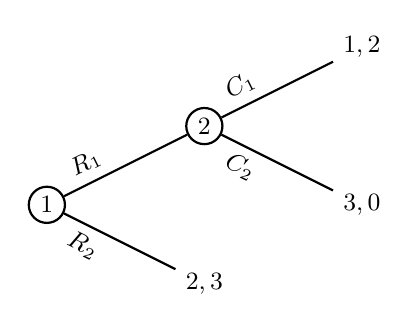
\begin{tikzpicture}[thick,
    circ/.style={circle,draw,thick,inner sep=2pt,font=\small},
    end/.style={font=\small},
    leftlabel/.style={above,sloped,near start,font=\small},
    rightlabel/.style={below,sloped,near start,font=\small},
    every label/.style={font=\small}]
  \node[circ] (1) at (0,0) {1}; % node (1)
  \node[circ] (2) at (2,1) {2}; % node (2)
  \node[end] (e23) at (2,-1) {$2,3$}; % end node: 2,3
  \node[end] (e30) at (4,0) {$3,0$};
  \node[end] (e12) at (4,2) {$1,2$};
  \draw (1) -- node[leftlabel] {$R_{1}$} (2); % line (1) -> (2)
  \draw (1) -- node[rightlabel] {$R_{2}$} (e23); % line (1) -> e23
  \draw (2) -- node[leftlabel] {$C_{1}$} (e12); % line (1) -> e23
  \draw (2) -- node[rightlabel] {$C_{2}$} (e30); % line (1) -> e23
\end{tikzpicture}
\end{center}

\cmnt{%
  If nodes are connected by dotted lines, then the relevant player
  cannot tell if she is in one of those nodes at which of them she
  is. Such nodes form an \emph{information set}. Games in which there
  can be ignorance about the present node are said to have
  \emph{imperfect information}.%
} %

% From a decision theoretic perspective, a game with several moves is a
% series of (potential) decision problems, one for each occasion where a
% player faces a choice. The states in these decision problems specify
% the future decisions of all players. As before, under the assumption
% that the utilities and rationality of players are common knowledge, we
% can often predict what will happen without specifying the players'
% degrees of belief.

We can use backward induction to predict how the game is going to be played,
assuming (1)--(3).

Consider node 2, where Column has a choice between outcome `3, 0' and outcome
`1, 2'. The choice involves no relevant uncertainty, and Column prefers `1, 2'
over `3, 0'. He can be expected to play $C_1$. Anticipating this, Row can figure
out that playing $R_1$ at node 1 will lead to `1, 2'. $R_{2}$ instead leads to `2,
3'. This is better for Row. So Row will play $R_2$.

In the following example, backward induction leads to a more surprising result.

\cmnt{%

  A game tree can be reduced to a simple decision matrix by pretending
  that all players decide at the outset on a \emph{strategy} that
  settles what they will choose at each point they might reach, with
  the constraint that the same choice must be made at each point in an
  information set. The resulting matrix is known as the
  \emph{strategic normal form} of the game tree.

  The outcome of an interaction often depends not only on their
  individual choices, but also on external matters, e.g. on whether
  some restaurant is open. Game theory accommodates this by using
  ``lotteries'' as outcomes. For instance, if I want to meet you, and
  we both end up at the restaurant, the outcome might be the complex
  state of affairs $\bet{\emph{Open}}{\emph{Meet \& Eat}}{\emph{Meet
      \& $\neg$Eat}}$. The utility of this state of affairs then
  depends on the probability that the restaurant is open. Since game
  theory tries to avoid specifying subjective probabilities, it is
  usually assumed that the relevant events have an objective chance
  which is common knowledge among all players. Thus it might be
  specified that all parties know that the restaurant owner each day
  decides whether to open her restaurant based on a fair coin toss.

  It's important to treat such games not in normal form. That's
  because the normal form ignores information that can arrive during a
  game. In particular, an agent might play something unexpected and
  this might change what the other agent should do.
} %

\begin{example}(Centipede)%
  You and Bob are playing a game. The game starts with a pot containing £2. In
  round 1, you can decide whether to continue or end the game. If you end the
  game, you get the £2 and Bob gets £0. If you continue, the money in the pot
  increases by £2 and Bob decides whether to continue or end. If he ends the
  game here (in round 2), the pot is divided so that he gets £3 and you get £1.
  If he continues, the money in the pot increases by another £2 and it's your
  turn again. If you end the game (in round 3), you get £4 and Bob gets £2. And
  so on. In each round, the money in the pot increases by £2 and whoever ends
  the game gets £2 more than the other player. In round 100, Bob no longer has
  an option to continue.
\end{example}
Suppose you and Bob don't care about each other; each of you only wants to get
as much money as possible. Here is a partial diagram of the resulting game.


\begin{center}
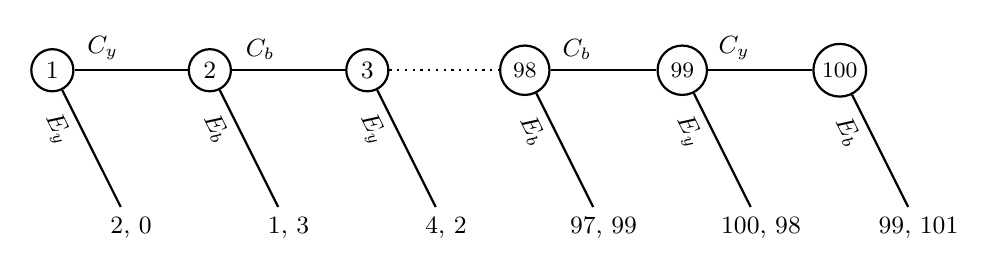
\begin{tikzpicture}[thick,
    p/.style={circle,draw,thick,inner sep=2pt,font=\small},
    xp/.style={circle,draw,thick,inner sep=2pt,font=\footnotesize},
    xxp/.style={circle,draw,thick,inner sep=2pt,font=\tiny},
    end/.style={font=\small},
    leftlabel/.style={above,sloped,near start,font=\small},
    rightlabel/.style={below,sloped,near start,font=\small},
    every label/.style={font=\small}]
  \node[p] (1) at (0,0) {\,1\,};
  \node[end] (1E) at (1,-2) {2, 0};
  \draw (1) -- node[rightlabel] {$E_{y}$} (1E);
  \node[p] (2) at (2,0) {\,2\,};
  \node[end] (2E) at (3,-2) {1, 3};
  \draw (2) -- node[rightlabel] {$E_{b}$} (2E);
  \draw (1) -- node[leftlabel] {$C_y$} (2);
  \node[p] (3) at (4,0) {\,3\,};
  \node[end] (3E) at (5,-2) {4, 2};
  \draw (3) -- node[rightlabel] {$E_{y}$} (3E);
  \draw (2) -- node[leftlabel] {$C_b$} (3);
  
  \node[xp] (98) at (6,0) {\,98\,};
  \node[end] (98E) at (7,-2) {97, 99};
  \draw[dotted] (3) -- (98);
  \node[xp] (99) at (8,0) {\,99\,};
  \node[end] (99E) at (9,-2) {100, 98};
  \draw (98) -- node[rightlabel] {$E_{b}$} (98E);
  \draw (98) -- node[leftlabel] {$C_b$} (99);
  \node[xp] (100) at (10,0) {100};
  \node[end] (100E) at (11,-2) {99, 101};
  \draw (99) -- node[rightlabel] {$E_{y}$} (99E);
  \draw (99) -- node[leftlabel] {$C_y$} (100);
  \draw (100) -- node[rightlabel] {$E_{b}$} (100E);
\end{tikzpicture}
\end{center}

Let's use backward induction to solve the game. At node 100, Bob doesn't have a
choice. If you continue at node 99 ($C_{y}$), you will get £99 and Bob £101. If
you end the game ($E_{y}$) at node 99, you will get £100. It is obviously better
to end the game. Anticipating this, what should Bob do in round 98? If he ends
the game ($E_b$), he'll get £99; if he continues ($C_b$), he'll get £98. So he
should end the game. Anticipating this, you should end the game in round 97, to
ensure that you'll get £98 rather than £97. And so on, all the way back to round
1. At each point, backward induction tells us that the game should be ended. In
particular, you can anticipate in round 1 that Bob will end the game in round 2.
So you should end the game in round 1. You will get £2 and Bob £0.

% \begin{exercise}{2}
%   Can you think of a real-life situation with a structure similar to
%   the centipede game? 
% \end{exercise}

When actual people play the Centipede game, almost no-one ends the game right
away. Is this a sign of either altruism or irrationality? Not necessarily.

Let's look at your choice in round 1 from an MEU perspective. It is clear what
happens if you end the game: you'll get £2. But what would happen if you chose
to continue? The argument from backward induction assumes that Bob would end the
game. If you could be certain that Bob would do that, then you should indeed end
the game in round 1. But why should Bob end the game? Because, so the argument,
he can be certain that you would end the game in round 3. But the argument for
ending in round 3 is exactly parallel to the argument for ending in round 1. And
if Bob faces a choice in round 2, then he has just seen that you \emph{did not}
end the game in round 1. Based on this information, he can't be sure you would
end it in round 3. On the contrary, he should be somewhat confident that you
will continue in round 3. And then continuing maximizes expected utility in
round 2. Anticipating this, continuing also maximizes expected utility in round
1, as it is likely to get you at least to round 3.

This suggests that the backward induction argument went wrong somewhere. But
where? Surely you really ought to end the game in round 99. And surely this
means that Bob should end the game in round 98. And so on! This puzzle is
sometimes called the \textbf{paradox of backward induction}.

\cmnt{%

  is what you would do if I were to play the ``wrong'' move. You would
  learn that either I'm not rational, or you're wrong about the
  utilities, or I believe that you're not rational or that you're
  wrong or that you believe that I'm wrong etc.

} %

% \begin{exercise}{2}
%   Consider a variant of the Centipede game with no fixed end point. Instead,
%   each time a player chooses to continue, the game ends with a probability of
%   1\%. Does this change anything? How should you play?
% \end{exercise}

\begin{exercise}{2}
  Suppose you repeatedly face the Prisoner's Dilemma with the same partner, for
  an unknown number of rounds. You only care about your own prison terms. You
  expect that your partner will remain silent in the first round and from then
  on imitate whatever you did in the previous round. What should you do? Does
  your answer show that you should choose a dominated act?
\end{exercise}


\section{Evolutionary game theory}

One of the most successful applications of game theory lies (somewhat
surprisingly) in the study of biological and cultural evolution. Consider the
following game.

\begin{example}(The Stag Hunt) Two players independently decide whether to hunt
  stag or rabbit. Hunting stag requires cooperation, so if only one of the
  players decides to hunt stag, she will get nothing. The utilities are as
  follows.
  
  \begin{dmatrix}{r|c|c}
       &  Stag &  Rabbit \\\hline
       Stag & 5, 5 & 0, 1 \\\hline
       Rabbit & 1, 0 & 1, 1 \\\hline
  \end{dmatrix}
  \vspace{-3mm}
\end{example}

In the evolutionary interpretation, the utilities represent the
\emph{relative fitness} that results from a combination of choices,
measured in terms of average number of surviving offspring. Let's
assume that each strategy is played by a certain fraction of
individuals in a population. Individuals who achieve an outcome with
greater utility will, by definition, have more offspring on average,
so their proportion in the population will increase.

Suppose initially $\nicefrac{1}{4}$ of the individuals in the population goes
for stags and $\nicefrac{3}{4}$ for rabbits. Assuming that encounters between
individuals are completely random, this means that any given individual has a
$\nicefrac{1}{4}$ chance of playing with someone hunting stag, and a
$\nicefrac{3}{4}$ chance of playing with someone hunting rabbit. The average
utility of hunting stag is
$\nicefrac{1}{4} \cdot 5 + \nicefrac{3}{4} \cdot 0 = 1.25$; for hunting rabbit
the utility is of course 1. Individuals going for stag have greater average
fitness. Their fraction in the population increases. As a consequence, it
becomes even more advantageous to go for stag. Eventually, everyone will hunt
stag.

By contrast, suppose initially only $\nicefrac{1}{10}$ of the population goes
for stags. Then hunting stag has an average utility of 0.5, which is less than
the utility of hunting rabbit. The rabbit hunters will have more offspring,
which makes it even worse to hunt stags. Eventually, everyone will hunt rabbits.

The two outcomes `Stag, Stag' and `Rabbit, Rabbit' are the two Nash Equilibria
in the Stag Hunt. Evolutionary game theory predicts that the proportion of stag
and rabbit hunters in a population will approach one of these equilibria.

\cmnt{%
  Notice that unlike in standard game theory, we made no assumptions
  about common knowledge here. The players don't have to know
  anything, and they can be quite irrational. That's because it's not
  the \emph{players} who decide which strategy is optimal and which
  equilibrium will be reached, but \emph{nature}. Individuals aren't
  actually trying to maximise fitness, but they nevertheless behave as
  if they were, because nature selects for individuals with higher
  fitness.
} %

\cmnt{%

  If you think of all possible fractions of strategies as a phase
  space, the equilibrium (Stag, Stag) has a larger basin of attraction
  than (Rabbit, Rabbit). Sometimes, a Nash equilibrium has a
  point-sized basin of attraction, such as $B, B$ in the following
  game:

  
    \begin{dmatrix}{r|c|c}
       &  A &  B \\\hline
       B & 5, 5 & 0, 0 \\\hline
       B & 0, 0 & 0, 0 \\\hline
    \end{dmatrix}
  

  It is very unlikely that this equilibrium could ever be found -- not
  only because it is unlikely that all players start off playing
  B. Rather, even in this case, mutants or intruders playing A will
  quickly take over. 

} %

Not every Nash Equilibrium is a possible end point of evolution though. If a
population repeatedly plays the game of Chicken, and the players can't recognize
in advance who will swerve and who will go straight, then the asymmetric
equilibria `Swerve, Straight' and `Straight, Swerve' do not mark possible end
points of evolutionary dynamics. But note that in a community in which almost
everyone swerves, you're better off going straight; similarly, in a community in
which almost everyone goes straight, the best choice is to swerve. Evolution
will therefore lead to the third, mixed strategy equilibrium. It will lead to a
state in which a certain fraction of the population swerves and the others go
straight.

\cmnt{%
  Hunting stag and hunting rabbit are \textbf{evolutionarily stable}
  in the sense that mutants playing the alternative strategy could not
  take over a population of 100\% stag hunters or 100\% rabbit
  hunters.
} %

\cmnt{%
  for all other strategies $Y$,
  \begin{itemize}
  \item \emph{either} $U(X,X) > U(Y,X)$,
  \item \emph{or} $U(X,X) = U(Y,X)$ and $U(X,Y) > U(Y,Y)$.
  \end{itemize}
  The idea is that either $X$ is \emph{strictly} better against itself
  than every alternative, or, if some mutant alternative $Y$ does
  equally good against $X$, then $X$ does better against $Y$ than $Y$
  itself. 
} %

\cmnt{%
  Considerations of mutants and invaders point at a limitation of our
  original dynamical model, which assumed that the ratios in the next
  generation are entirely determined by the ratios in the parent
  generation and their fitness, without mutation and invasion. There are
  more complex models including these factors.

  Notice that unlike in standard game theory, we made no assumptions
  about common knowledge here. The players don't have to know
  anything, and they can be quite irrational. That's because it's not
  the \emph{players} who decide which strategy is optimal and which
  equilibrium will be reached, but \emph{nature}. Individuals aren't
  actually trying to maximise fitness, but they nevertheless behave as
  if they were, because nature selects for individuals with higher
  fitness.

  What exactly is fitness in evolutionary game theory? It is best
  defined by its role: fitness is something such that the more you
  have it, the more creatures like you will exist in the next
  generation. An obvious candidate is number of offspring, but there
  are situations where this isn't adequate, e.g. when the players are
  ants or more generally when players have a choice that helps other
  players of their type to have more offspring. Biologists sometimes
  speak of ``inclusive fitness'' to take such factors into account.
} %

The assumption that individuals in a population are randomly paired with one
another is obviously an idealisation. In reality, individuals are more likely to
interact with members of their own family, which increases the chances that they
will be paired with individuals of the same type; they might also actively seek
out others who share the relevant traits. Either way, the resulting
\textbf{correlated play} dramatically changes the picture.

Imagine a population in which individuals repeatedly play a Prisoner's Dilemma
wherein they can either cooperate (remain silent, in the original scenario) or
defect (confess). Since defectors do better than cooperators in any encounter,
it may seem that cooperation can never evolve. On the other hand, cooperators do
much better when paired with other cooperators than defectors when paired with
defectors. If the extent of correlation is sufficiently high, cooperators can
take over (although perhaps not completely).

In many species, one can find altruistic individuals who sacrifice
their own fitness for the sake of others. Evolutionary game theory
explains how this kind of altruism could have evolved.

% \begin{exercise}{1}
%   Why can't we expect cooperative behaviour to take over completely in
%   the scenario where cooperation spreads through correlated play?
%  \end{exercise}

\begin{exercise}{1}
  What are the Nash equilibria in the following game (ignoring
  randomization)? Could all the equilibria come about through an
  evolutionary process? 
  \vspace{-1mm}
  
    \begin{dmatrix}{r|c|c}
       &  A &  B \\\hline
       A & 5, 5 & 1, 1 \\\hline
       B & 1, 1 & 1, 1 \\\hline
    \end{dmatrix}
  \vspace{-2mm}
  
\end{exercise}

\begin{essay}
  Explain the paradox of backward induction. Why is it a paradox? How
  do you think it could be resolved?
\end{essay}

\begin{sources}

  There are many decent introductions to Game Theory. The
  \href{https://plato.stanford.edu/entries/game-theory/}{``Game Theory''} entry
  in the Stanford Encyclopedia by Don Ross (2019) provides a fairly
  comprehensive overview. A suitable next step might be Steven Tadelis,
  \emph{Game Theory: An Introduction} (2013).

  The paradox of backward induction is discussed, for example, in Philip Pettit
  and Robert Sugden, ``The Backward Induction Paradox'' (1989).

  For a little more on evolutionary game theory, see Brian Skyrms, ``Game
  Theory, Rationality and Evolution of the Social Contract'' (2000). For even
  more, see Brian Skyrms, ``The Stag Hunt and the Evolution of Social
  Structure'' (2004).
  
\end{sources}



%%% Local Variables: 
%%% mode: latex
%%% TeX-master: "bdrc.tex"
%%% End:
